\documentclass{article}
\usepackage[utf8]{inputenc}

\usepackage{enumitem}
\usepackage{amsmath}
\usepackage{amssymb}
\usepackage{graphicx}
\usepackage[colorinlistoftodos]{todonotes}
\usepackage[colorlinks=true, allcolors=blue]{hyperref}
\usepackage{caption}
\usepackage{subcaption}
%\usepackage{sectsty}
%\usepackage{apacite}
\usepackage{float}
\usepackage{titling} 
\usepackage{blindtext}
\usepackage[square,sort,comma,numbers]{natbib}
\usepackage[colorinlistoftodos]{todonotes}
\usepackage{xcolor}
\usepackage{indentfirst}
\usepackage{amsmath}
\usepackage{mathtools}
\usepackage{tabularx}
\usepackage{array}
\usepackage[linesnumbered,algoruled,boxed,lined]{algorithm2e}
\setlength\parskip{.5\baselineskip plus .1\baselineskip  minus .1\baselineskip}
\setlength{\parindent}{1em}

\title{MVA - Project}
\author{Hongping Feng, Pau Rodriguez, Wangyang Ye }
\date{June 2018}

\begin{document}

\maketitle

\section{Introduction}
Thyroid is an interminable and complex infection happened because of unseemly TSH (Thyroid Simulating Hormone) levels or might be brought on by the issues in thyroid organ itself. The most widely recognized reason for hypothyroidism is hashimoto's thyroid. It is an auto safe condition where the body makes antibodies that pulverize the thyroid organ. The system behind the flow of the event of the thyroid ailment is still not completely caught on. The consequences related to thyroid disease are growing rapidly and provides new insights into the biological mechanism involved and helps in the management of thyroid disease. 

The  controlling  of  digestion  system  helps  organs  like  the heart, work appropriately. In any case, the disease of thyroid  must  discharge  a  fitting  measure  of  hormones  into the circulatory system. This movement controlled by the pituitary organ, which produces Thyroid Stimulating Hormone  (TSH),  stimulates  not  animated  the  arrival  of  both  T4  and  T3.  At the point when  thyroid  over  produces  and  exorbitantly  secretes  hormones, this condition is hyperthyroidism (overactive thyroid).   The   inverse   situation   when   hormones   are   inadequately  created  and  discharged  is  hypothyroidism  (under  dynamic  thyroid).  Hypothyroidism  causes  the  majority  of  the  body’s  procedures  to  back  off  and  may  expand  heart  assault  hazard  due  to  uplifted  cholesterol  levels.  A  portion  of  the  more  regular  hormonal  issue  is  connected with the thyroid organ, which is a piece of the endocrine framework. this framework is about gathering of  organs  that  emit  chemicals  called  hormones  specifically into the circulation system. 

Here, we applied Random Forest algorithm in identifying the thyroid dysfunctionality over with the \textit{Thyroid Disease Data Set} in UCI Machine Learning Repository. 

This directory contains the latest version of an archive of thyroid diagnoses
obtained from the Garvan Institute, consisting of 9172 records from 1984 to
early 1987.  Each record has 29 attributes and 1 response variable (diagnosis to multi classes). The attributes are given in order and separated by commas.  Unknown attribute values are indicated by question marks.  The varaiables are:
\begin{center}
\begin{tabular}{c | c }
\textbf{Attribute Name} & \textbf{Possible Values}  \\ \hline
age & continuous \\
sex & M, F \\
on thyroxine & f, t \\
query on thyroxine & f, t \\
on antithyroid medication & f, t \\
sick & f, t \\
pregnant & f, t \\
thyroid surgery & f, t \\
I131 treatment & f, t \\sick & f, t \\
query hypothyroid & f, t \\
query hyperthyroid & f, t \\
lithium & f, t \\
goitre & f, t \\
tumor & f, t \\
hypopituitary & f, t \\
psych & f, t \\
TSH measured & f, t \\
TSH & continuous \\
T3 measured & f, t \\
T3 & continuous \\
TT4 measured & f, t \\
TT4 & continuous \\
T4U measured & f, t \\
T4U & continuous \\
FTI measured & f, t \\
FTI & continuous \\
TBG measured & f, t \\
TBG & continuous \\
referral source & WEST, STMW, SVHC, SVI, SVHD, other\\
class & -, A-T
\end{tabular}
\label{table:cvalue1}
\end{center}

The diagnosis consists of a string of letters indicating diagnosed conditions. A diagnosis "-" indicates no condition requiring comment. The
conditions are divided into groups where each group corresponds to a class of comments.

\begin{center}
\begin{tabular}{c | c }
\textbf{Letter} & \textbf{Diagnosis}  \\ \hline
& \textbf{hyperthyroid conditions} \\
A & hyperthyroid \\
B & T3 toxic \\
C & toxic goitre \\
D & secondary toxic \\ \hline

& \textbf{hypothyroid conditions} \\
E & hypothyroid \\
F & primary hypothyroid \\
G & compensated hypothyroid \\
H & secondary hypothyroid \\ \hline

& \textbf{binding protein} \\
I & increased binding protein \\
J & decreased binding protein \\ \hline

& \textbf{general health} \\
K & concurrent non-thyroidal illness \\ \hline

& \textbf{replacement therapy} \\
L & consistent with replacement therapy \\
M & underreplaced \\
N & overreplaced \\ \hline

& \textbf{antithyroid treatment} \\
O & antithyroid drugs \\
P & I131 treatment \\
Q & surgery \\ \hline

& \textbf{miscellaneous} \\
O & discordant assay results \\
P & elevated TBG \\
Q & elevated thyroid hormones \\ \hline

\end{tabular}
\label{table:cvalue1}
\end{center}

\section{Data Pre-processing}

Our preprocessing consisted in setting continuous variables as numeric, and categorical variables as factors.

\textbf{Errors:} we detected 3 individuals with an incorrect value for the age variable ( a value of 65535 which is clearly an error). We removed those individuals as they proportion in the dataset is very small.\\
\textbf{Missing values:} Several of the continuous variables related to measurements on blood tests have missing values. One of them, called TBG, is specially important since  8823 individuals out of 9169 have this value as missing. Looking on information about the test associated with this variable, we see that it is an important measurement but that it is not usually done. We also learn that the range of values for a healthy person is between 10 mg\/100 mL and 24 mg\/100 mL. Looking at the summary of this variable within individuals where the value is not missing, we see that the mean in the dataset is 29.87, and that the mean for individuals with the class "-" (which means they don't have a condition) is 22.9, whereas for the individuals that have any of the conditions it is  47.72.\\ At that point we had three different options to proceed: to remove the variable, to impute the individuals that do not have a condition with the mean for the TBG variable of the individuals that don't have a condition and the rest with an iterative imputation algorithm like Mice, and finally to impute all with the Mice iterative algorithm. We execute the three approaches and compared the resulting first factorial plane in PCA and the contribution of that variable TBG to the first principal component, to see if the the variable TBG carries an important amount of inertia. If this variable carries an important amount of inertia, it cannot be remove from the dataset.
% PCA contributions

\begin{figure}[H]
\minipage{0.5\textwidth}%
  \centering
  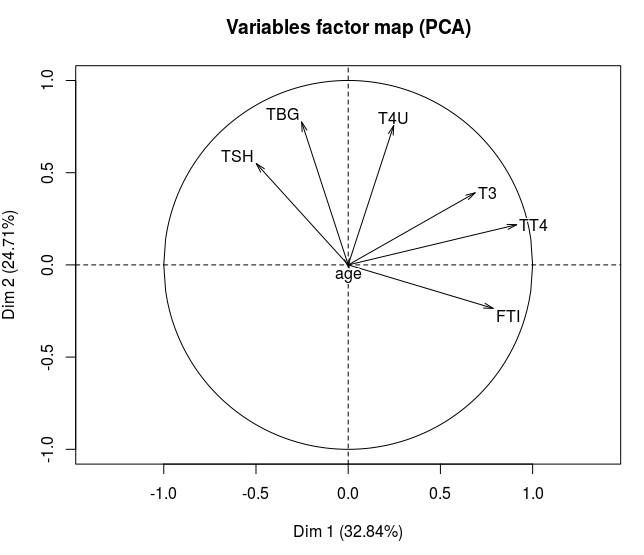
\includegraphics[width=\linewidth]{img/Missing_all_1f.png}
  \caption{Imputation with Mice}\label{missing_contrib1}
\endminipage\hfill
\minipage{0.5\textwidth}%
  \centering
  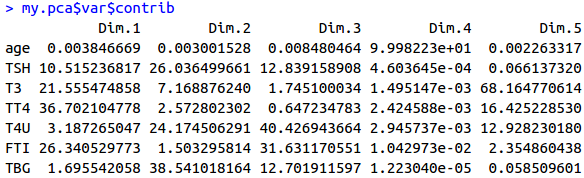
\includegraphics[width=\linewidth]{img/MIssing_imputecondition_contrib.png}
  \caption{Combined imputaton}\label{missing_contrib2}
\endminipage
\caption{Different approaches on imputation (all with Mice or combined) , then showing contribution of TBG variable to PC}
\end{figure}
%\vspace*{-15pt}

With the result of the contributions to the first principal components and the amount of inertia explained by both principal components we decide that this variable must be considered in the analysis as it carries an important amount of inertia.\\
We also compared the two approaches where TBG is totally imputed or just imputed on the individuals that suffer from a condition, to see which of the two imputation strategies affect or disturb the final result or they are in fact similar. We suspected that, since healthy individuals are usually not tested by TBG, using the mean of the TBG variable for healthy individuals on healthy individuals that have this value missing is the most correct thing to do. 
% PCA results
\begin{figure}[H]
\minipage{0.5\textwidth}%
  \centering
  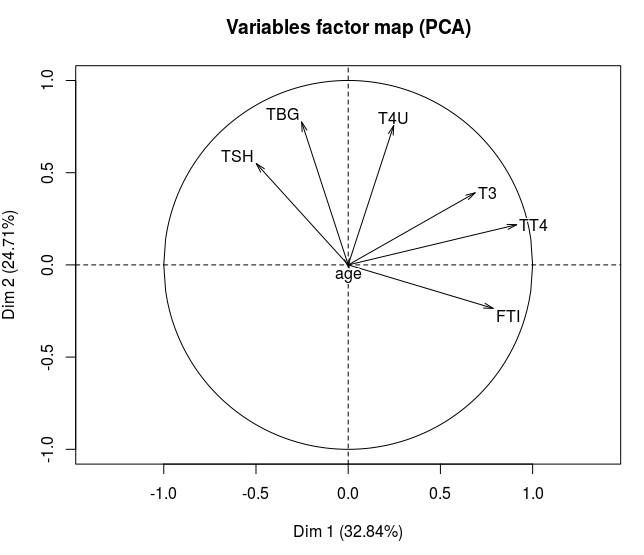
\includegraphics[width=\linewidth]{img/Missing_all_1f.png}
  \caption{Imputation with Mice}\label{missing_contrib1}
\endminipage\hfill
\minipage{0.5\textwidth}%
  \centering
  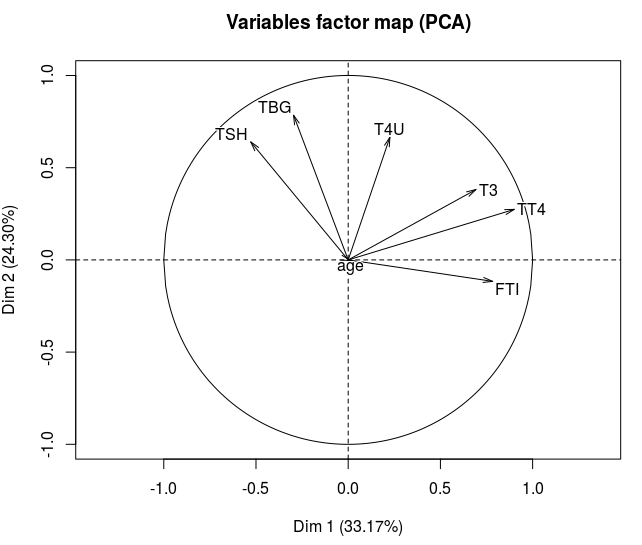
\includegraphics[width=\linewidth]{img/MIssing_imputecond1_1f.png}
  \caption{Combined imputaton}\label{missing_contrib2}
\endminipage
\caption{First factorial plane with different approaches on imputation (all with Mice or combined)}
\end{figure}
%\vspace*{-15pt}

We observe that the imputation with Mice for all individual is very close to the combined imputation. Therefore, to stay closer to real values we impute all the missing values with Mice.

\textbf{Outliers:}

\section{Validation Protocol}

\section{Interpretation of Latent Concepts}

\section{Clustering}

\section{Interpretation of Clusters}

\section{Discussion}

\section{Prediction}

\section{Conclusion}


\end{document}
